\documentclass[english,man,doc,11pt, twoside,floatsintext]{apa6}
\usepackage{lmodern}
\usepackage{amssymb,amsmath}
\usepackage{ifxetex,ifluatex}
\usepackage{fixltx2e} % provides \textsubscript
\ifnum 0\ifxetex 1\fi\ifluatex 1\fi=0 % if pdftex
  \usepackage[T1]{fontenc}
  \usepackage[utf8]{inputenc}
\else % if luatex or xelatex
  \ifxetex
    \usepackage{mathspec}
  \else
    \usepackage{fontspec}
  \fi
  \defaultfontfeatures{Ligatures=TeX,Scale=MatchLowercase}
\fi
% use upquote if available, for straight quotes in verbatim environments
\IfFileExists{upquote.sty}{\usepackage{upquote}}{}
% use microtype if available
\IfFileExists{microtype.sty}{%
\usepackage{microtype}
\UseMicrotypeSet[protrusion]{basicmath} % disable protrusion for tt fonts
}{}
\usepackage{hyperref}
\hypersetup{unicode=true,
            pdftitle={Thesis proposal: Diffusion of innovation in sustainability in a context of Dutch energy transition},
            pdfauthor={Marco Bunt},
            pdfkeywords={keywords},
            pdfborder={0 0 0},
            breaklinks=true}
\urlstyle{same}  % don't use monospace font for urls
\ifnum 0\ifxetex 1\fi\ifluatex 1\fi=0 % if pdftex
  \usepackage[shorthands=off,main=english]{babel}
\else
  \usepackage{polyglossia}
  \setmainlanguage[]{english}
\fi
\usepackage{graphicx,grffile}
\makeatletter
\def\maxwidth{\ifdim\Gin@nat@width>\linewidth\linewidth\else\Gin@nat@width\fi}
\def\maxheight{\ifdim\Gin@nat@height>\textheight\textheight\else\Gin@nat@height\fi}
\makeatother
% Scale images if necessary, so that they will not overflow the page
% margins by default, and it is still possible to overwrite the defaults
% using explicit options in \includegraphics[width, height, ...]{}
\setkeys{Gin}{width=\maxwidth,height=\maxheight,keepaspectratio}
\IfFileExists{parskip.sty}{%
\usepackage{parskip}
}{% else
\setlength{\parindent}{0pt}
\setlength{\parskip}{6pt plus 2pt minus 1pt}
}
\setlength{\emergencystretch}{3em}  % prevent overfull lines
\providecommand{\tightlist}{%
  \setlength{\itemsep}{0pt}\setlength{\parskip}{0pt}}
\setcounter{secnumdepth}{0}
% Redefines (sub)paragraphs to behave more like sections
\ifx\paragraph\undefined\else
\let\oldparagraph\paragraph
\renewcommand{\paragraph}[1]{\oldparagraph{#1}\mbox{}}
\fi
\ifx\subparagraph\undefined\else
\let\oldsubparagraph\subparagraph
\renewcommand{\subparagraph}[1]{\oldsubparagraph{#1}\mbox{}}
\fi

%%% Use protect on footnotes to avoid problems with footnotes in titles
\let\rmarkdownfootnote\footnote%
\def\footnote{\protect\rmarkdownfootnote}


  \title{Thesis proposal: Diffusion of innovation in sustainability in a context
of Dutch energy transition}
    \author{Marco Bunt\textsuperscript{1,2}}
    \date{}
  
\shorttitle{Diffusion of innovation in sustainability}
\affiliation{
\vspace{0.5cm}
\textsuperscript{1} Erasmus school of social and behavioural sciences\\\textsuperscript{2} Stedin netbeheer}
\keywords{keywords\newline\indent Word count: X}
\usepackage{csquotes}
\usepackage{upgreek}
\captionsetup{font=singlespacing,justification=justified}

\usepackage{longtable}
\usepackage{lscape}
\usepackage{multirow}
\usepackage{tabularx}
\usepackage[flushleft]{threeparttable}
\usepackage{threeparttablex}

\newenvironment{lltable}{\begin{landscape}\begin{center}\begin{ThreePartTable}}{\end{ThreePartTable}\end{center}\end{landscape}}

\makeatletter
\newcommand\LastLTentrywidth{1em}
\newlength\longtablewidth
\setlength{\longtablewidth}{1in}
\newcommand{\getlongtablewidth}{\begingroup \ifcsname LT@\roman{LT@tables}\endcsname \global\longtablewidth=0pt \renewcommand{\LT@entry}[2]{\global\advance\longtablewidth by ##2\relax\gdef\LastLTentrywidth{##2}}\@nameuse{LT@\roman{LT@tables}} \fi \endgroup}



\authornote{This article is the graduation thesis om Marco
Bunt for the study social science on the Erasmus school of social and
behavioral sciences, in collaboration with Stedin.

Correspondence concerning this article should be addressed to Marco
Bunt, Stedin, Blaak 8, 3011 TA Rotterdam. E-mail:
\href{mailto:marco.bunt@Stedin.net}{\nolinkurl{marco.bunt@Stedin.net}}}

\abstract{
Yet to be written


}

\begin{document}
\maketitle

\section{Introduction}\label{introduction}

Climate change urge national and local governments to make policy's to
enable energy transition from fossil energy sources that are free from
emitting carbon in the atmosphere(Economische Zaken en Klimaat, 2019).
Governments hold differed tactics in pushing society towards a
sustainable future, such as 1) punishing bad behavior. 2) rewarding good
behavior, 3) use social influence or norms to influence public opinion
and 4) persuasion by marked stimuli (Salazar, Oerlemans, \&
Stroe-Biezen, 2012). The Dutch municipalities have chosen the last
option. Via a web of subsidies citizens are persuaded to invest in
sustainable technology(Energiesubsidiewijzer.nl, n.d.). Question arises:
\emph{What publics are not addressed in the persuasive tactics of the
government to push energy transition via marked stimuli?} The aim of
this article is evaluate this policy by investigating in what areas in
the Dutch society are not infiltrated by new sustainable technology.
Thereby this research adds a new perspective on the Dutch energy
transition, since it is investigating what groups in the Dutch society
are not adopting to energy solutions to prevent climate change.

The topic is already investigated in a opposite direction, and concluded
that the annual income of the household end the peer-effects are the
best predictors in prediction the adaptation of new sustainable
technology. There are qualitative articles investigating the discursive
trends in post-foundational democracy in transition management (Jhagroe
\& Loorbach, 2015), but no quantitative analysis is done on the mutual
characteristics of people that are not transitioning their energy
consumption to sustainable sources. A difficult factor in this research,
is the \enquote{Naive Psychology} in investigating the peer-effect of
the spread of sustainable technology, since people seems unable to
detect the effect of normative social influence. In many cases, people
underestimate the effect that the norms of their peers.

Much research is contributed to explaining the diffusion of innovation
{[}ToDo Spatial diffusion of innovation{]}, as well as the diffusion of
sustainable technology's by households(Hyysalo \& Usenyuk, 2015; Salazar
et al., 2012).

\section{Problem statement}\label{problem-statement}

\begin{figure}

{\centering 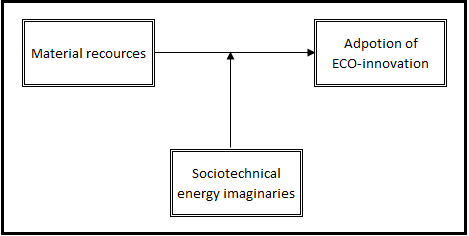
\includegraphics[width=4.05in]{C:/Users/602956/Desktop/Studie/Thesis/Sociology thesis/Conceptueel model/ConceptueelModel} 

}

\caption{Conceptual model adoptation of sustainable technology}\label{fig:knit}
\end{figure}

\section{Theoretical framework}\label{theoretical-framework}

\section{Methods and data}\label{methods-and-data}

\newpage

\section{References}\label{references}

\begingroup
\setlength{\parindent}{-0.5in} \setlength{\leftskip}{0.5in}

\hypertarget{refs}{}
\hypertarget{ref-klimaat_2019}{}
Economische Zaken en Klimaat, M. van. (2019, January). Klimaatakkoord.
\emph{Klimaatakkoord}. Ministerie van Economische Zaken en Klimaat.
Retrieved from \url{https://www.klimaatakkoord.nl/}

\hypertarget{ref-energiesubsidiewijzer}{}
Energiesubsidiewijzer.nl. (n.d.). Kan ik subsidie krijgen voor
energiebesparing? Doe hier de check! \emph{Kan ik subsidie krijgen voor
energiebesparing? Doe hier de check! - Energiesubsidiewijzer.nl}.
Retrieved from \url{https://www.energiesubsidiewijzer.nl/}

\hypertarget{ref-hyysalo_2015}{}
Hyysalo, S., \& Usenyuk, S. (2015). The user dominated technology era:
Dynamics of dispersed peer-innovation. \emph{Research Policy},
\emph{44}(3), 560--576.
doi:\href{https://doi.org/10.1016/j.respol.2015.01.002}{10.1016/j.respol.2015.01.002}

\hypertarget{ref-jhagroe_2015}{}
Jhagroe, S., \& Loorbach, D. (2015). See no evil, hear no evil: The
democratic potential of transition management. \emph{Environmental
Innovation and Societal Transitions}, \emph{15}, 65--83.
doi:\href{https://doi.org/10.1016/j.eist.2014.07.001}{10.1016/j.eist.2014.07.001}

\hypertarget{ref-salazar_2012}{}
Salazar, H. A., Oerlemans, L., \& Stroe-Biezen, S. V. (2012). Social
influence on sustainable consumption: Evidence from a behavioural
experiment. \emph{International Journal of Consumer Studies},
\emph{37}(2), 172--180.
doi:\href{https://doi.org/10.1111/j.1470-6431.2012.01110.x}{10.1111/j.1470-6431.2012.01110.x}

\endgroup


\end{document}
